\subsection{API}
	La componente API è il core dell'intera architettura; permette all'applicazione web di interfacciarsi con i due database menzionati precedentemente, oltre che con un \glock{bot Telegram}.
	\newline
	La componente è stata sviluppata in Java 11, utilizzando dei \glock{framework Spring}: Spring boot, Spring security, Spring Kafka e Spring jpa; per l'autenticazione web è stato usato Json Web Token.

	\subsubsection{Diagramma dei package}%%%%%%%%%%%%%%OK
		\begin{figure}[H]
			\centering
			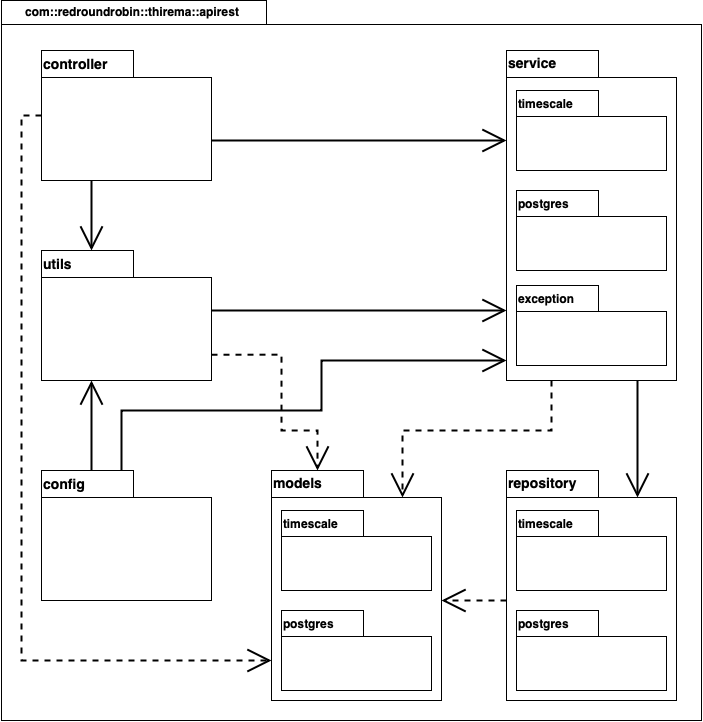
\includegraphics[scale=0.500]{res/images/API/packageAPI.png}
			\caption{Diagramma dei packages per la componente API}
			\label{Diagramma 10}
		\end{figure}

	\subsubsection{Dipendenze esterne}
		La componente API he le seguenti dipendenze esterne:
		\begin{itemize}
			\item \textbf{Spring Boot:} che viene utilizzato per rendere le \glock{API} un microservizio; 
			\item \textbf{Spring Boot Jpa:} contenuta nel framework precedente, viene utilizzata per permettere al package Repository e Config di interfacciarsi direttamente con il database;
			\item \textbf{Spring Boot Starter Security:} contenuta nel framework Spring Boot, viene utilizzata per gestire la sicurezza nell'accesso alle \glock{API};
			\item \textbf{SpringBoot Starter Test:} contenuta nel framework Spring Boot, viene utilizzata per eseguire i test;
			\item \textbf{org.Moquito:} libreria usata per fare simulare il comportamento di alcune funzioni, in fase di test;
			\item \textbf{io.jsonwebtoken:} libreria usata per la creazione di token necessari all'accesso ad aree riservate delle \glock{API};
			\item \textbf{Spring Kafka:} libreria utilizzata per la comunicazione con \glock{Kafka};
			\item \textbf{Spring Doc:} libreria utilizzata per la visualizzazione delle richieste \glock{API} tramite interfaccia web;
			\item \textbf{org.postgreSql.Driver:} che viene utilizzato per la connessione con DBMS di tipo Postgre.
		\end{itemize}

	\subsubsection{Diagrammi delle classi}
		Al fine di semplificare la comprensione delle dipendenze della componente \glock{API}, si è deciso di suddividere i diagrammi per package, mostrando in dettaglio quelli più significativi.
		\newpage
		\paragraph*{Package Utils}
		\begin{figure}[H]
			\centering
			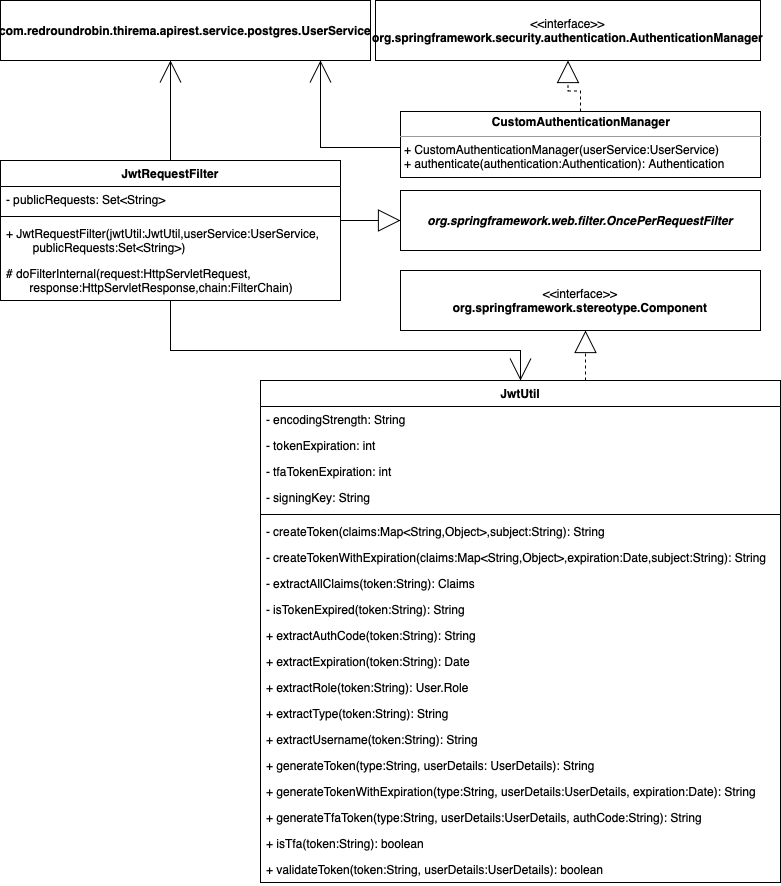
\includegraphics[scale=0.550]{res/images/API/UtilsPackage.png}
			\caption{Diagramma del package utils della componente API}
			\label{Diagramma 11}
		\end{figure}
		\newpage
		All'interno del package Utils sono presenti le seguenti classi:
		\begin{itemize}
			\item \textbf{JwtRequestFilter}: la classe dipende dalle classi UserService e JwtUtils ed estende la classe OncePerRequestFilter, permettendo di filtrare le richieste effettuate dal bot Telegram o dalla Web-app verso le \glock{API};
			\item \textbf{JwtUtil}: la classe implementa l'interfaccia Component del \glock{framework spring}. Più nel dettaglio la classe JwtUtil permette di gestire i token: è posssibile infatti creare varie tipologie di token che permettono l'autenticazione e la richiesta di dati alle API. Sempre all'interno di questa classe è presente un metodo per verificare l'autenticità di un certo token;
			\item \textbf{CustomAuthenticationManager}: questa classe dipende da UserService ed implementa l'interfaccia AuthenticationManager del framework Spring, permettendo quindi la gestione e la personalizzazione dell'autenticazione.
		\end{itemize}
		
		\newpage
		\paragraph*{Package Config} 
		\begin{figure}[H]
			\centering
			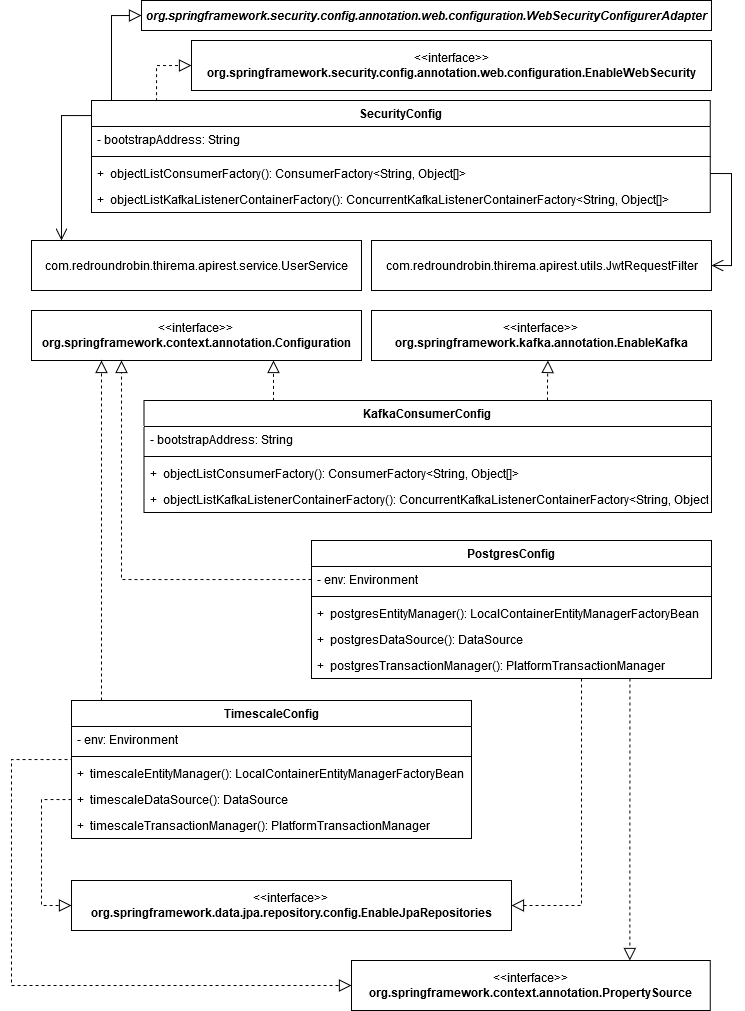
\includegraphics[scale=0.550]{res/images/API/ConfigPackage.png}
			\caption{Diagramma del package config della componente API}
			\label{Diagramma 12}
		\end{figure}
		\newpage
		Il diagramma del package Config mostra le dipendenze delle classi di configurazione della componente \glock{API}.
		\newline
		Il package Config contiene le classi in cui vengono effettuate le configurazioni di deiverse componenti delle API. Sono infatti presenti:
		\begin{itemize}
			\item \textbf{PostgresConfig} e \textbf{TimescaleConfig}: queste classi vengono utilizzate per configurare l'accesso ai nostri database ed implementano le interfacce PropertySource, JpaRepository e Configuration del framework Spring;
			\item \textbf{KafkaConsumerConfig}: questa classe viene utilizzata per configurare l'accesso al broker Kafka contenuto all'interno del sistema. Per poter essere implementata ha bisogno delle dipendenze verso le interfacce Configuration ed EnableKafka del framework Spring;
			\item \textbf{SecurityConfig}: questa classe viene utilizzata per configurare i servizi di sicurezza impiegati dalle API, e permettere o meno ad alcune richieste HTTP di accedere a questa componente. Ha delle dipendenze verso UserService e WebSecurityAdapter mentre implementa l'interfaccia EnableWebSecurity.
		\end{itemize}
		\newpage
		\paragraph*{Package Controllers}

		Il package Controllers visualizzabile all'interno del file \textit{Immagini/API-PackageController.png} contiene i controller per mappare le richieste GET e POST che è possibile ricevere da parte della \glock{web app} o di \glock{Telegram}.
		\newline
		Ogni classe per poter funzionare implementa l'interfaccia RequestMapping e RestController del framework Spring. Inoltre estendono la classe astratta CoreController che permette di gestire le varie autorizzazioni che hanno gli utenti per effettuare o meno una certa richiesta.
		Le classi presenti nel package sono le seguenti:
		\begin{itemize}
			\item \textbf{EntityController}: permette di gestire le richieste che riguardano i dati da reperire o inserire dal database per quanto riguarda gli enti presenti nel sistema. Contiene un riferimento ad EntityService;
			\item \textbf{ViewController}: permette di gestire le richieste che riguardano la gestione della configurazioni di una o più view all'interno della omonima sezione della Web-app. Contiene un riferimento a ViewService;
			\item \textbf{ViewGraphController}: permette di gestire le richieste che riguardano le configurazioni dei vari grafici presenti all'interno di una specifica view all'interno della Web-app. Contiene un riferimento a ViewGraphService;
			\item \textbf{DataController}: permette di gestire le richieste che riguardano il reperimento di valori di un determinato sensore presenti all'interno del database Timescale. Contiene un riferimento a SensorService;
			\item \textbf{SensorController}: permette di gestire le richieste che riguardano i sensori salvati all'interno del database relazionale. A differenza di DataController questa classe non è incentrata sul raccogliere i dati dei sensori. Contiene un riferimento a SensorService;
			\item \textbf{DeviceController}: permette di gestire le richieste che riguardano il reperimento dei dispositivi e sensori sulla base di un certo ente o id di un certo dispositivo. Contiene un riferimento SensorService e DeviceService;
			\item \textbf{GatewayController}: permette di gestire le richieste che riguardano i vari Gateway presenti nel sistema; Per ogni gateway è possibile reperire i dispositivi ed i sensori. Contiene un riferimento a DeviceService, GatewayService e SensorService;
			\item \textbf{UserController}: permette la gestione delle richieste che riguardano la creazione, eliminazione e gestione dei dati degli utenti presenti nel sistema; 
			\item \textbf{AuthController}: questa classe permette di gestire le richieste che riguardano l'autenticazione (sia normale che 2FA) degli utenti all'interno della Web-app o del bot Telegram. Contiene un riferimento verso CustomAuthenticationManager e TelegramService.  
		\end{itemize}
		\paragraph*{Package Models}
		\newpage
		\begin{figure}[H]
			\centering
			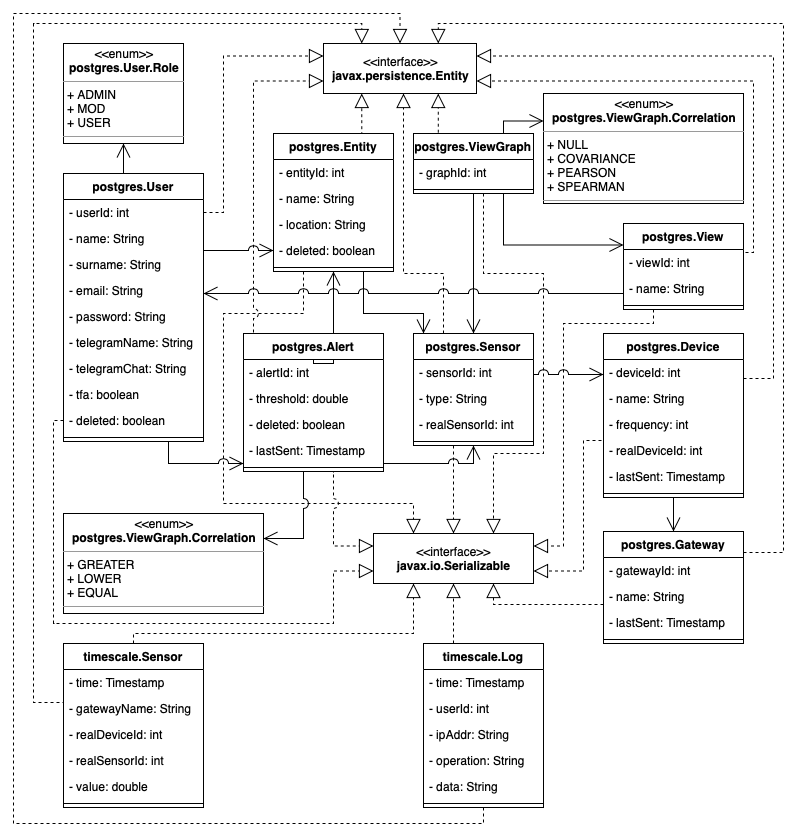
\includegraphics[scale=0.550]{res/images/API/ModelsPackage.png}
			\caption{Diagramma del package models della componente API}
			\label{Diagramma 14}
		\end{figure}
		Nel diagramma in alto vengono descritte le dipendenze del package Models, che rappresentano le relazioni che ci sono fra le varie entità del database relazionale.
		Le classi presenti nel diagramma sono le seguenti:
		\begin{itemize}
		 	\item \textbf{postgres.User}: rappresenta l'entità User e le sue relazioni all'interno del database relazionale. Implementa le interfacce Serializable e javax.persistence.Entity e possiede un riferimento a postgres.User.Role;
		 	\item \textbf{postgres.Entity}: rappresenta l'entità Entity e le sue relazioni all'interno del database relazionale. Implementa le interfacce Serializable e javax.persistence.Entity e possiede un riferimento a postgres.Sensor;
		 	\item \textbf{postgres.Gateway}: rappresenta l'entità Gateway all'interno e le sue relazioni del database relazionale. Implementa le interfacce Serializable e javax.persistence.Entity;
		 	\item \textbf{postgres.View}: rappresenta l'entità view e le sue relazioni all'interno del database relazionale. Implementa le interfacce Serializable e javax.persistence.Entity e possiede un riferimento a postgres.User;
		 	\item \textbf{postgres.Sensor}: rappresenta l'entità Sensor e le sue relazioni all'interno del database relazionale. Implementa le interfacce Serializable e javax.persistence.Entity e possiede un riferimento a postgres.Device;
		 	\item \textbf{postgres.Device}: rappresenta l'entità Device e le sue relazioni all'interno del database relazionale. Implementa le interfacce Serializable e javax.persistence.Entity e possiede un riferimento a postgres.Gateway;
		 	\item \textbf{postgres.Alert}: rappresenta l'entità Alert e le sue relazioni all'interno del database relazionale. Implementa le interfacce Serializable e javax.persistence.Entity e possiede dei riferimenti a postgres.Entity e postgres.Sensor;
		 	\item \textbf{postgres.Viewgraph}: rappresenta l'entità ViewGraph e le sue relazioni all'interno del database relazionale. Implementa le interfacce Serializable e javax.persistence.Entity e possiede dei riferimenti a postgres.View e postgres.ViewGraph.Correlation;
		 	\item \textbf{postgres.ViewGraph.Correlation}: rappresenta l'entità Correlation di un certo grafico e le sue relazioni all'interno del database relazionale. Implementa le interfacce Serializable e javax.persistence.Entity;
		 	\item \textbf{postgres.User.Role}: rappresenta l'entità Role di un determinato utente e le sue relazioni all'interno del database relazionale. Implementa le interfacce Serializable e javax.persistence.Entity;
		 	\item \textbf{timescale.Sensor}: rappresenta l'entità Sensor all'interno del database non relazionale. Implementa le interfacce Serializable e javax.persistence.Entity;
		 	\item \textbf{timescale.Log}: rappresenta l'entità Log all'interno del database non relazionale. Implementa le interfacce Serializable e javax.persistence.Entity.
		 \end{itemize} 
		\begin{landscape}
		\paragraph*{Package Repository}
		\begin{figure}[H]
			\centering
			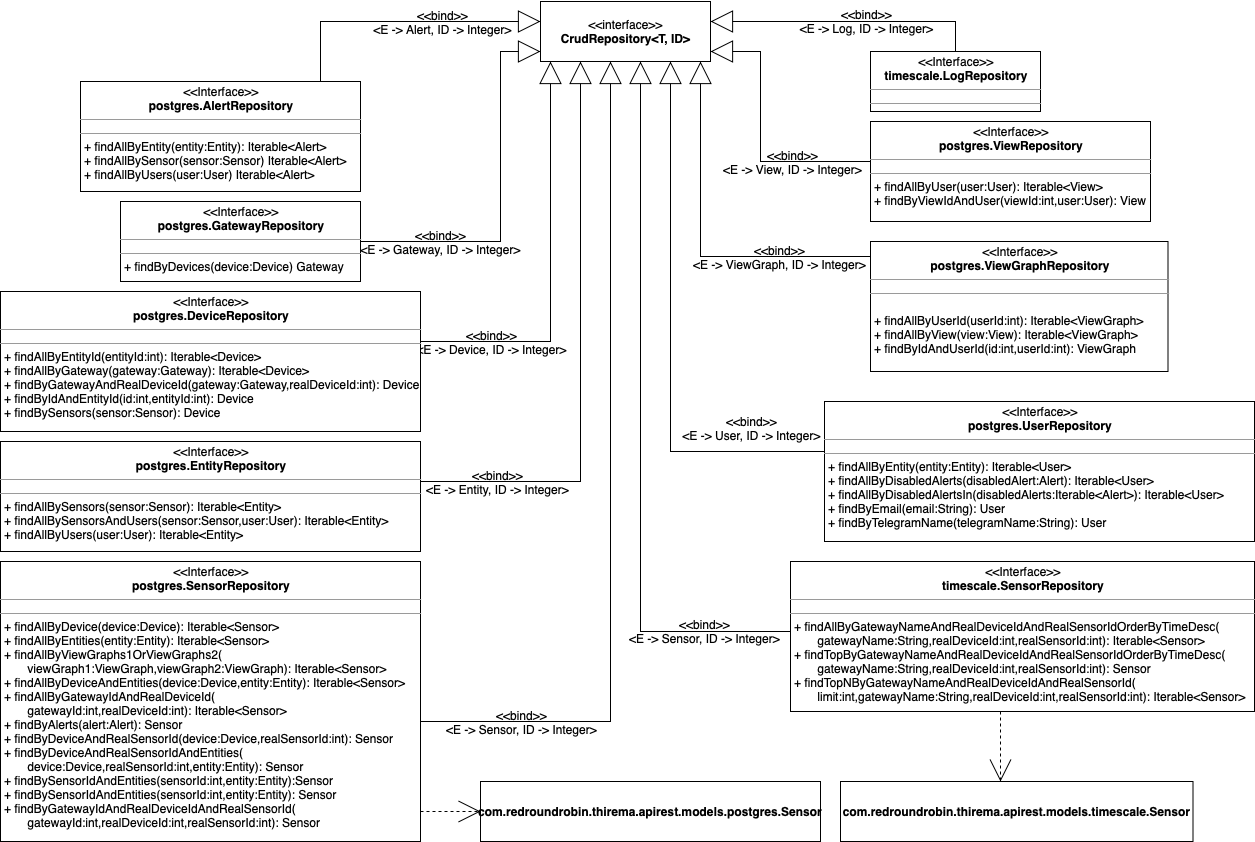
\includegraphics[scale=0.500]{res/images/API/RepositoryPackage.png}
			\caption{Diagramma del package repository della componente API}
			\label{Diagramma 15}
		\end{figure}
		Nel diagramma che rappresenta le dipendenze del package Repository della componente \glock{API}, sono presenti le interfacce che rappresentano le query che vengono effettuate a database nelle varie tabelle. Tutte le interfacce estendono l'interfaccia CrudRepository.
		Le interfacce presenti del package rappresentato dal diagramma sono:
		\begin{itemize}
			\item \textbf{postgres.AlertRepository}: questa interfaccia rappresenta le query che è possibile fare per reperire gli alert per uno specifico ente, sensore o utente;
			\item \textbf{postgres.GatewayRepository}: questa interfaccia rappresenta le query che è possibile fare per reperire il gateway a partire da uno specifico dispositivo;
			\item \textbf{postgres.DeviceRepository}: questa interfaccia rappresenta le query che è possibile fare per reperire i dispositivi a partire da un ente, un sensore o da un identificativo;
			\item \textbf{postgres.EntityRepository}: questa interfaccia rappresenta le query che è possibile fare per reperire un ente a partire dai suoi sensori associati o dai suoi utenti;
			\item \textbf{postgres.SensorRepository}: questa interfaccia rappresenta le query che è possibile fare per reperire uno o più sensori a partire da un dispositivo, un ente, una view, un gateway o un alert. Oltre ad estendere l'interfaccia CrudRepository utilizza anche la classe models.postgres.Sensor;
			\item \textbf{postgres.UserRepository}: questa interfaccia rappresenta le query che è possibile fare per reperire uno o più utenti a partire da un ente, email o username Telegram oppure dall'avere o meno degli alert disabilitati;
			\item \textbf{postgres.ViewGraphRepository}: questa interfaccia rappresenta le query che è possibile fare per reperire i grafici a partire da un utente o da una vista;
			\item \textbf{timescale.LogRepository}: questa interfaccia rappresenta le query che è possibile fare per reperire i log all'interno del database non relazionale;
			\item \textbf{timescale.SensorRepository}: questa interfaccia rappresenta le query che è possibile fare per reperire i dati di un sensore a partire dal nome del gateway e dall'id del sensore.
		\end{itemize}
		\paragraph*{Package Service}
		Nel diagramma delle classi all'interno del file \\ \textit{Immagini/API-PackageService.png} che rappresenta il package Service sono rappresentate classi che effettuano le query a database ad un livello di astrazione più alto rispetto al package Repository. Quest'ultimo viene infatti utilizzato dai service per effettuare le query a database.
		Ogni classi del package Service implementa l'interfaccia Service del framework Spring.
		Le classi presenti nel package rappresentato nel diagramma sono le seguenti:
		\begin{itemize}
			\item \textbf{postgres.ViewService}: questa classe permette di reperire dati relativi alle View dal database relazionale. Ha dei riferimenti verso ViewRepository e UserRepository;
			\item \textbf{postgres.ViewgraphService}: questa classe permette di reperire dati relativi ai grafici relativi ad una view dal database relazionale. Ha dei riferimenti verso ViewRepository, ViewGraphRepository e SensorRepository;
			\item \textbf{postgres.SensorService}: questa classe permette di reperire dati relativi ai sensori dal database relazionale. Ha dei riferimenti verso ViewgraphRepository, SensorRepository, AlertRepository ed EntityRepository;
			\item \textbf{TelegramService}: questa classe permette di reperire dati relativi all'autenticazione a due fattori o all'invio di comandi dal database relazionale. Contiene un riferimento a RestTemplate del framework Spring;
			\item \textbf{postgres.GatewayService}: questa classe permette di reperire dati relativi ai gateway dal database relazionale. Possiede dei riferimenti verso GatewayRepository e DeviceRepository;
			\item \textbf{postgres.EntityService}: questa classe permette di reperire dati relativi agli enti dal database relazionale. Possiede dei riferimenti a EntityRepository, UserRepository e SensorRepository;
			\item \textbf{postgres.DeviceService}: questa classe permette di reperire dati relativi ai dispositivi  dal database relazionale. Possiede dei riferimenti verso DeviceRepostory, GatewayRepository, EntityRepository e SensorRepository;
			\item \textbf{postgres.AlertService}: questa classe permette di reperire dati relativi agli alert dal database relazionale. Possiede dei riferimenti versoAlertRepository, EntityRepository, UserRepository e SensorRepository;
			\item \textbf{postgres.UserService}: questa classe permette di reperire dati relativi agli utenti dal database relazionale. Possiede dei riferimenti verso UserRepository, AlertRepository ed EntityRepository. Inoltre estende l'interfaccia UserDetailService del framework Spring;
			\item \textbf{timescale.LogService}: questa classe permette di reperire dati relativi ai logs di sistema dal database non relazionale. Ha un riferimento all'interfaccia LogRepository;
			\item \textbf{timescale.SensorService}: questa classe permette di reperire dati relativi ai dati di Timescale dei sensori immagazzinati nel database relazionale. Ha infatti due riferimenti distinti: uno verso postgres.SensorRepository ed uno verso timescale.SensorRepository;
		\end{itemize}
	
	\subsubsection{Diagrammi di sequenza}%%%%%%%%%OK
		\begin{figure}[H]
			\centering
			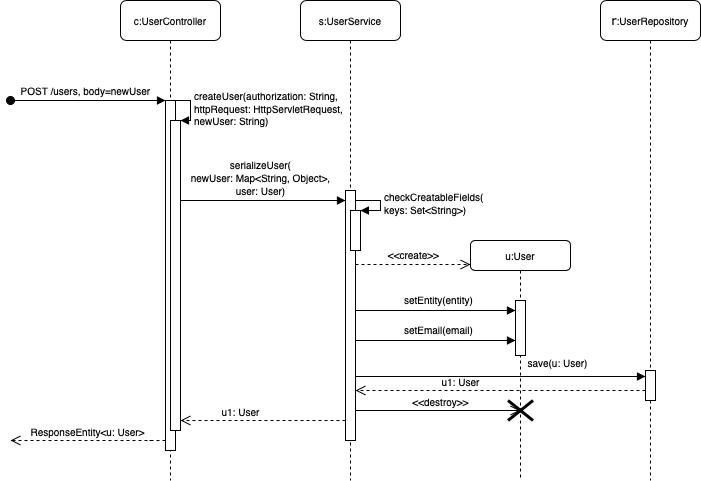
\includegraphics[scale=0.600]{res/images/API/inserimento_utente.png}
			\caption{Diagramma di sequenza che mostra l'inserimento di un utente all'interno della componente API}
			\label{Diagramma 17}
		\end{figure}
		Nel diagramma di sequenza in alto, alla ricezione di una richiesta POST dalla \glock{web app}, lo UserController chiede allo UserService di inserire un nuovo utente, dopo aver verificato che la richiesta provenisse da un utente con l'autorizzazione necessaria a crearne uno nuovo.
		\newline
		Viene creata poi un'istanza di User che, dopo averne impostato i campi, viene inviata a UserRepository, chiedendone il salvataggio nel database. Viene infine restituita l'entità inserita ed inviata in risposta alla \glock{web app} in formato \glock{JSON}.
		\begin{figure}[H]
			\centering
			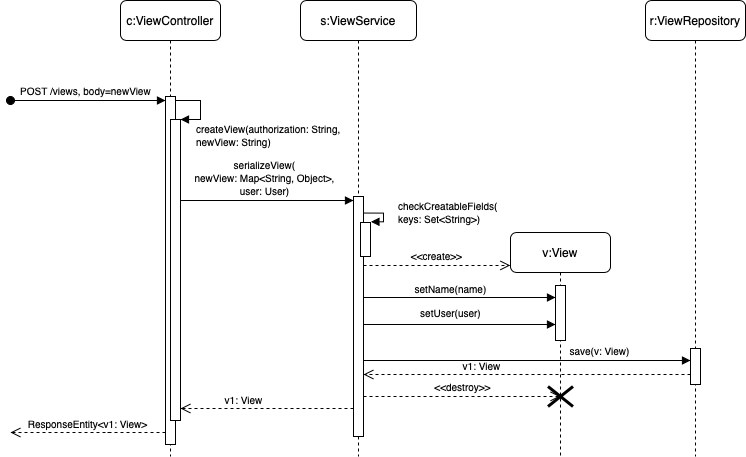
\includegraphics[scale=0.600]{res/images/API/inserimento_view.png}
			\caption{Diagramma di sequenza che mostra l'inserimento di una view all'interno della componente API}
			\label{Diagramma 18}
		\end{figure}
		Il diagramma descrive l'inserimento di una view all'interno del database. Il procedimento inserito è molto simile a quello descritto per l'inserimento di un utente.
	\end{landscape}
	

	\subsubsection{Documentazione OpenAPI}

	Per le API è stato generato un documento in formato OpenAPI con un file YAML. Questo documento è stato convertito in PDF per comodità di lettura, e contiene tutte le specifiche delle API realizzate con le relative chiamate e i relativi codici di errore in risposta.
	\newline
	I file in questione si possono trovare ai seguenti percorsi:
	\begin{itemize}
		\item \verb!OpenAPI/riot-api.v1.pdf! - documento PDF descrittivo di tutte le API realizzate;
		\item \verb!OpenAPI/riot-api.v1.yaml! - documento in formato YAML auto-generato tramite Spring.
	\end{itemize}
	
	\subsubsection{Estensione}
		\paragraph{Aggiungere una richiesta API}
			Per inserire una nuova richiesta, se non si usano le classi già esistenti, è necessario che la nuova classe creata implementi l'interfaccia RestController, tramite la notazione \textit{@RestController}, da inserire precedentemente alla definizione della classe.
			\newline
			All'interno della classe è necessario definire una funzione usando una notazione di tipo mapping, ad esempio "@GetMapping", inserendo all'interno delle parentesi tonde la stringa associata all'URI della richiesta che si vuole implementare.
			Ad esempio:
			\begin{verbatim}
			@GetMapping(value = \{"/{deviceId:.+}/sensors"\})
			\end{verbatim}
			Per esporre una risorsa senza necessità di autenticazione è necessario aggiungere all'array publicRequests l'URL della richiesta. L'array publicRequests è un attributo della classe SecurityConfig.